\section{Introduction}
The White Rabbit PTP Core is an Ethernet MAC implementation capable of providing
precise timing. It can be used for sending and receiving regular Ethernet
frames between user-defined HDL modules and a physical medium. It also
implements the White Rabbit protocol to provide sub-nanosecond time
synchronization.

The White Rabbit PTP Core can operate in one of the following modes:
\begin{itemize}
  \item GrandMaster: WR Master synchronized to an external 1-PPS and 10 MHz clock
    signal, propagates precise timing to other WR-compliant devices
  \item Master: WR Master with free-running oscillator, propagates precise
    timing to other WR-compliant devices
  \item Slave: synchronizes its internal oscillator to another WR Master device
\end{itemize}
By default it starts as \emph{Slave} but its mode can be changed in anytime
using the \emph{mode} command of WRPC Shell (please check the \emph{White
Rabbit PTP Core User's Manual - Building and Running} \cite{wrpc_man}  for full
description of the WRPC Shell).\\


This documentation describes the input and output ports of the WRPC IP-core and
VHDL generic parameters that can be used to personalize the core. The manual is
divided into two parts:
\begin{itemize}
  \item {\bf Part I: Standard configuration}: describes only generics and ports
    that have to be connected to use WRPC as the precise time source and be able
    to send and receive Ethernet frames through it.
  \item {\bf Part II: Advanced options}: all the generics and input/output ports
    that are beyond WRPC's basic usage. They can be used by people with expert
    knowledge of the White Rabbit and {\bf on their own responsibility} (the WRPC
    instantiated with those parameters modified won't be supported).
\end{itemize}

Figure \ref{intro:fig:wrpc_top} is an example on how to instantiate the WRPC
component inside the VHDL project. It contains few additional modules besides
the WRPC:
\begin{itemize}
  \item \emph{wr\_gtp\_phy\_spartan6}: module wrapping Xilinx GTP SerDes to
    improve its determinism
  \item \emph{PLL\_BASE}: Xilinx Spartan6 PLL primitive \cite{pll_base}, used to
    produce 62.5 MHz system clock from 125 MHz local reference clock and to
    produce the DMTD offset clock from a local 20 MHz oscillator
  \item \emph{spec\_serial\_dac\_arb}: converts DACs tuning values to serial
    interface and arbitrates access to two DACs used for reference and DMTD
    clock tuning.
\end{itemize}

%Very similar example can be found in the WRPC
%reference design for PCI-Express SPEC board:
%\emph{top/spec\_1\_1/wr\_core\_demo/spec\_top.vhd} inside \emph{wr-cores} git
%repository.

\begin{figure}[hbp]
  \begin{center}
    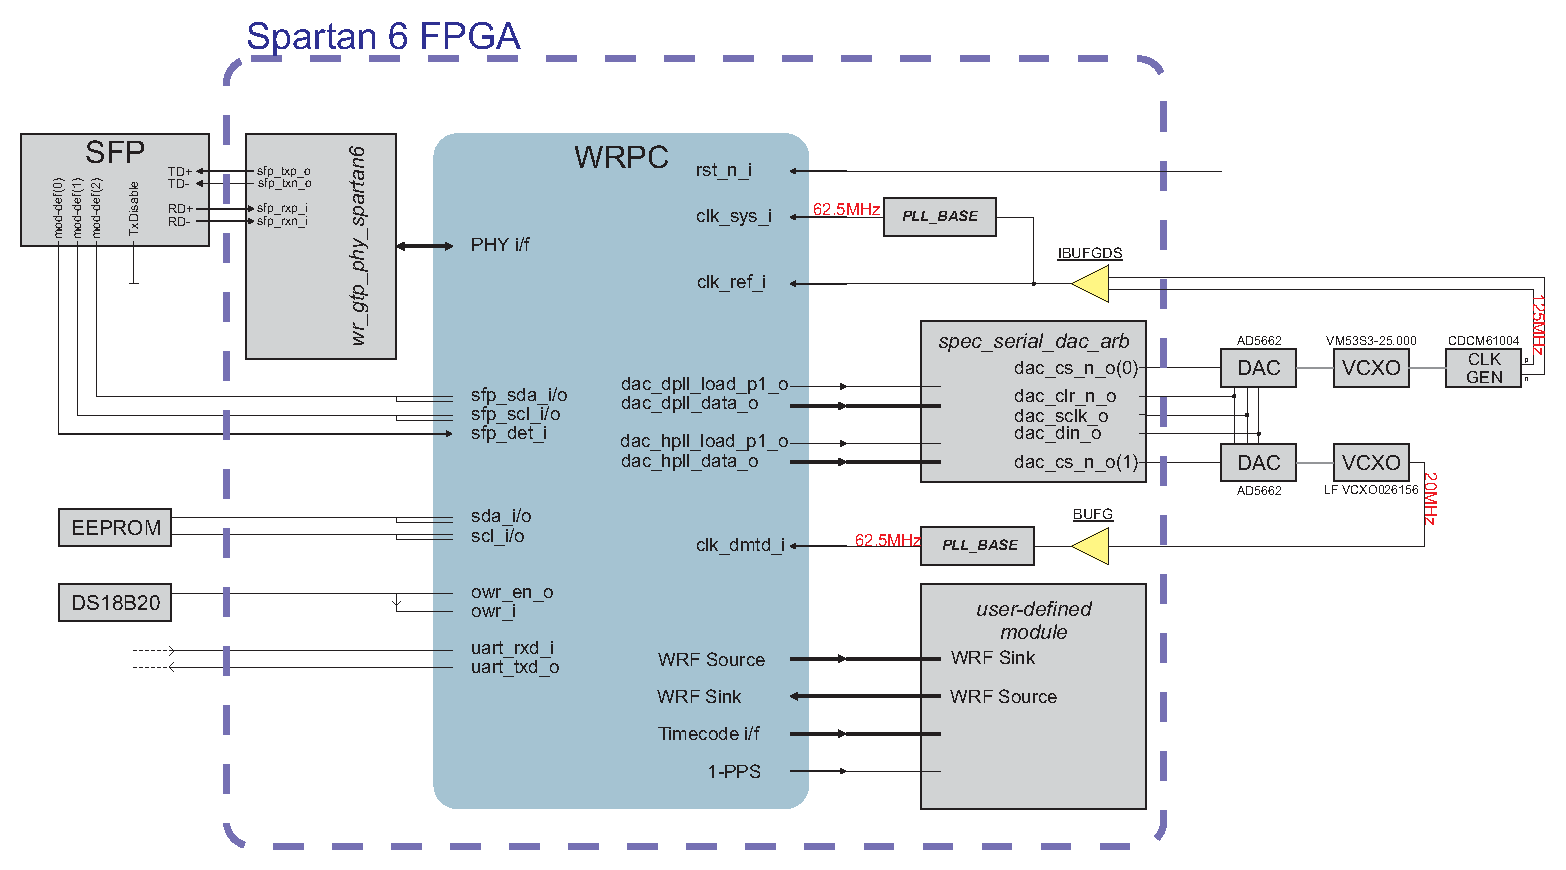
\includegraphics[width=.9\textheight, angle=270]{fig/basic_top.pdf}
    \label{intro:fig:wrpc_top}
    \caption{Simple top design with WRPC}
  \end{center}
\end{figure}

